\documentclass[10pt,mathserif]{beamer}
\usepackage{graphicx,amsmath,amssymb,tikz,psfrag}
\usepackage{hyperref}
\usepackage{subcaption}

\usepackage{psfrag,amsfonts,verbatim}
\usepackage{amsthm}

\input defs.tex
\input slide_format.tex

%% begin presentation

\title{\large \bfseries Discovering signals in fMRI data; 
a Bayesian nonparametric approach }

\author{Ahmed Bou-Rabee, Wanrong Zhu, Zheng Xu, Mo Zhou\\[3ex]
STAT 30850\\
University of Chicago}

\date{\today}

\begin{document}

\frame{
\thispagestyle{empty}
\titlepage
}

\begin{frame} {Project Goal}
\BIT
\item  Formulate a method which can adaptively identify clusters of signals in functional magnetic resonance imaging (fMRI) data.
\item  Evaluate the proposed method by drawing comparison between it and the existing p-filter algorithm.
\EIT
\end{frame}

\begin{frame} {What is fMRI data?}
\BIT
\item  fMRI data measures the change in brain blood flow associated with mental activity [HSM04].
\item  fMRI data is in the form (voxel, time, intensity of reading).
\item  Example: To identify regions of the brain associated with hunger, fMRI readings can be taken while hungry subjects are shown pictures of food.
\item  Multiple comparison problem due to hundreds of thousands of voxels 
\item  Identify significant clusters (not just individual voxels)
\EIT
\end{frame}

\begin{frame} {What's our method}
\BIT
\item  Inspired by Stephens (2000), we describe a bayesian nonparametric method by creating a Markov birth-death process with stationary distribution to detect clusters of signals. 
\item View each cluster as a point in parameter space.
\item Posterior distribution of the parameters being stationary distribution.
\item Theoretically, this method works for multiple-dimensional data which incorporates spatial and temporal information.

\EIT
\end{frame}

\begin{frame} {Details of the Method: Priors}
\BIT
\item number of signal clusters:  $k \sim \mbox{Truncated Poisson}(\lambda,  1, k_{max})$.
\item signal centers:   $c_j \sim U \mathcal{(D)}$ for $j = 1, ... , k$.
\item signal radius:  $r_j \sim \mbox{Truncated Normal}(\mu,\sigma,r_{min},r_{max}) \mbox{ for j = 1, \ldots k} $.
\item signal strength:  $\beta_j \sim U(\beta_{min},\beta_{max}) \mbox{ for j = 1, \ldots, k} $.
\item p-values in signal clusters:  $p_i \sim Beta(\frac{1}{\beta_j}, \beta_j)$, when $x_i$ is in cluster $j$.
\item p-values not in signal clusters:  $p_i \sim U(0,1)$.
\EIT
\end{frame}

\begin{frame} {Details of the Method (continued): inventing the chain}
\BIT
\item Birth: generating a new cluster.
\item Death: "killing" an existing cluster.
\item Birth rate: constant $\lambda$ is pre-defined and independent of clusters.
\item Death rate: $\mu_i$ depends on "current" clusters and is updated each step.
\item Flip a weighted coin to decide birth (w/ prob $\frac{\lambda}{\lambda+\mu_i}$) or death (w/ prob $\frac{\mu_i}{\lambda+\mu_i}$).
\EIT
\end{frame}

\begin{frame} {Details of the Method (continued): death rate calculation using likelihoods}
\BIT 
\item $K$ clusters with prior $Beta(\frac{1}{\beta_j}, \beta_j)$ for $j = 1,2, ..., K$. K itself is random with prior $F_K$.
\item Label specify which cluster each data point belongs.
\item Current cluster likelihood: $l = log L(data | Beta(\frac{1}{\beta_j}, \beta_i)'s, labels)$; $c = logL(K | F_K)$
\item Cluster likelihood after "killing" cluster j: $l_{-j} = log L(data | Beta(\frac{1}{\beta_j}, \beta_i)'s, labels_{-j})$; $c_{-j} = logL(K-1 | F_K)$
\item $u_j$ = $log(\lambda) + (l_{-j} - l) + (c_{-j} - log(K) - c)$ for $j = 1,2, ..., K$.
\item $u$ = $\sum_{j=1}^K e^{u_j}$.
\EIT
\end{frame}

\begin{frame} {Details of the Method (continued)}
\BIT 
\item At the end of each step, run metropolis-hasting algorithm to sample from the posterior of the beta distribution
\item Purpose: TODO

\EIT 
\end{frame}

\begin{frame} {Details of the Method (continued)}
\BIT 
\item Run the chain long enough before starting collect sample labels.
\item Sample labels from evenly space grid along the chain to avoid autocorrelation.
\item Average over sample labels to determine if it is signal or null.
\EIT 
\end{frame}

\begin{frame} {Toy Data: Preliminaries}
\BIT
\item 100-by-100 grid with $k$=5 clusters of signals and the rest is null.
\item The centers $C_k \sim$  uniform from the grid while being distinct for $k = 1, 2, ..., 5$
\item The radius $R_k \sim T N (7, 2, 5, 10)$ for $k = 1, 2, ..., 5$
\item Signals in clusters $p_{ki} \sim Beta(1, \beta_k)$ where $\beta_k \sim TN(8, 5, 2, 200)$ for $k = 1, 2, ..., 5$
\EIT
\end{frame}

\begin{frame} {Toy Data (continued): Performance }
\begin{figure}[t!]
    \centering
    \begin{subfigure}[t]{0.3\textwidth}
        \centering
        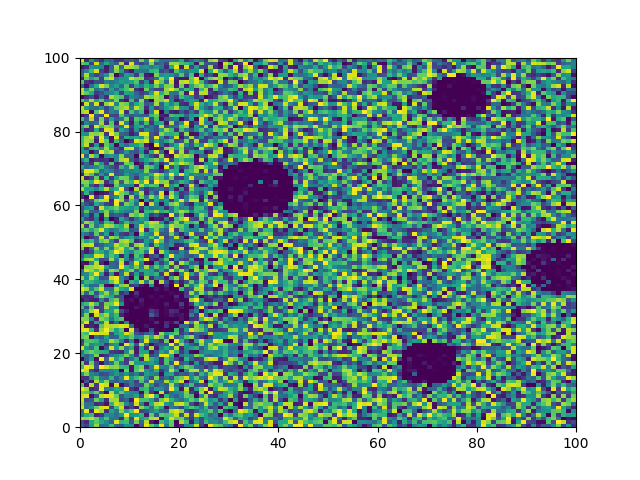
\includegraphics[height=1.2in, width=1.4in]{../BDC_gridactual}
        \caption{Actual grid}
    \end{subfigure}%
    \begin{subfigure}[t]{0.3\textwidth}
        \centering
        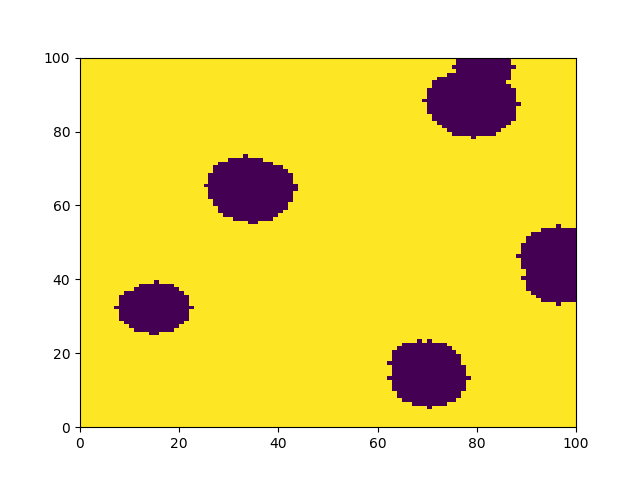
\includegraphics[height=1.2in, width=1.4in]{../BDC_grid1}
        \caption{Birth death chain}
    \end{subfigure}%
    \begin{subfigure}[t]{0.3\textwidth}
        \centering
        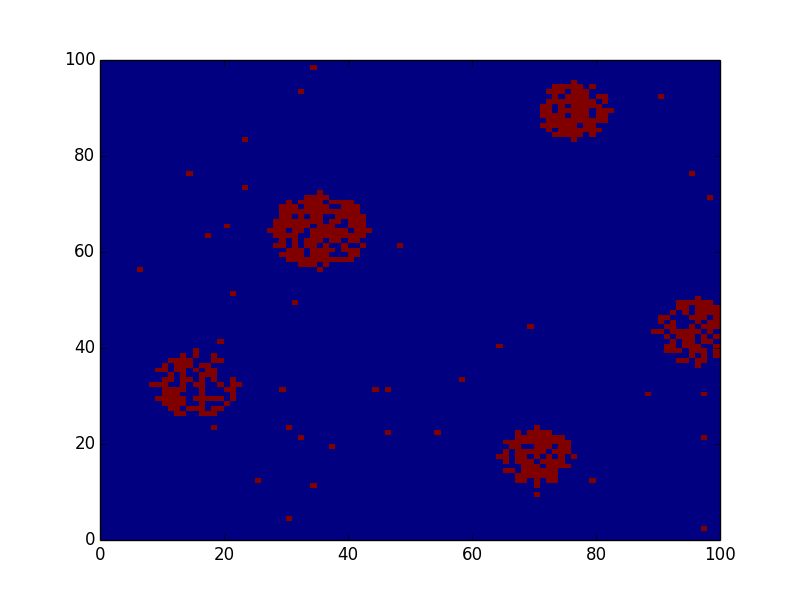
\includegraphics[height=1.2in, width=1.4in]{../BH_toy_data}
        \caption{p-filter}
    \end{subfigure}
    \caption{Simulated data}
\end{figure}
\end{frame}


\begin{frame}{Toy Data (continued): More on Priors}
\begin{figure}[t!]
    \centering
    \begin{subfigure}[t]{0.3\textwidth}
        \centering
        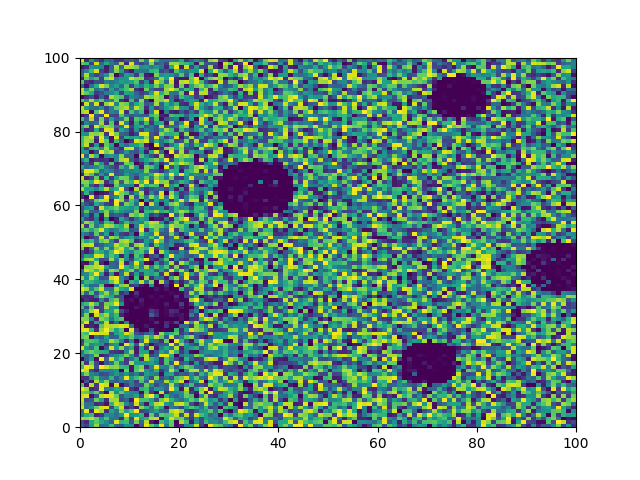
\includegraphics[height=1.2in, width=1.4in]{../BDC_gridactual}
        \caption{Actual grid}
    \end{subfigure}%
    \begin{subfigure}[t]{0.3\textwidth}
        \centering
        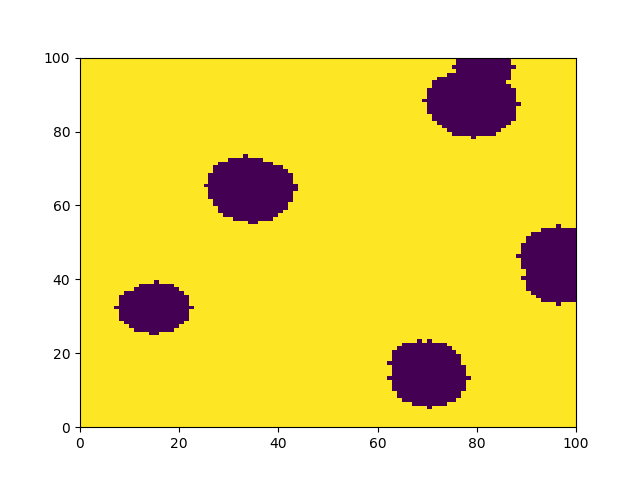
\includegraphics[height=1.2in, width=1.4in]{../BDC_grid1}
        \caption{$k \sim Trun(Poi(50), 1, 100)$; $r \sim TN(7, 2, 5, 10)$; $\beta \sim TN(8, 5, 2, 200)$}
    \end{subfigure} %
    \caption{Simulated data}
\end{figure}
\end{frame}


\begin{frame}{Toy Data (continued): More on Priors}
First, let's compare different priors on beta
\begin{figure}[t!]
    \centering
    \begin{subfigure}[t]{0.3\textwidth}
        \centering
        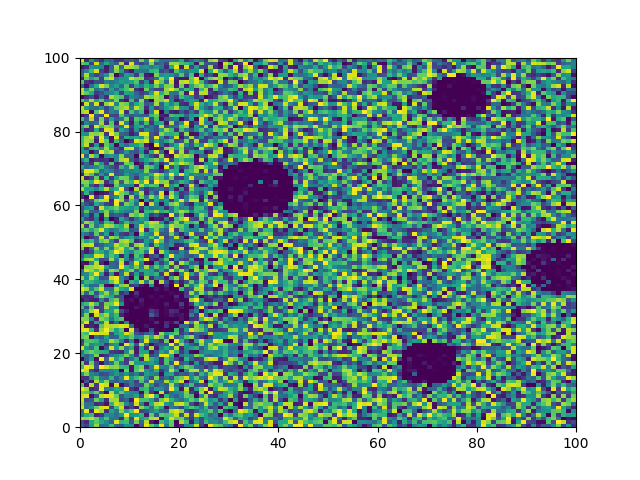
\includegraphics[height=1.3in, width=1.4in]{../BDC_gridactual}
        \caption{Actual grid}
    \end{subfigure}%
    \begin{subfigure}[t]{0.3\textwidth}
        \centering
        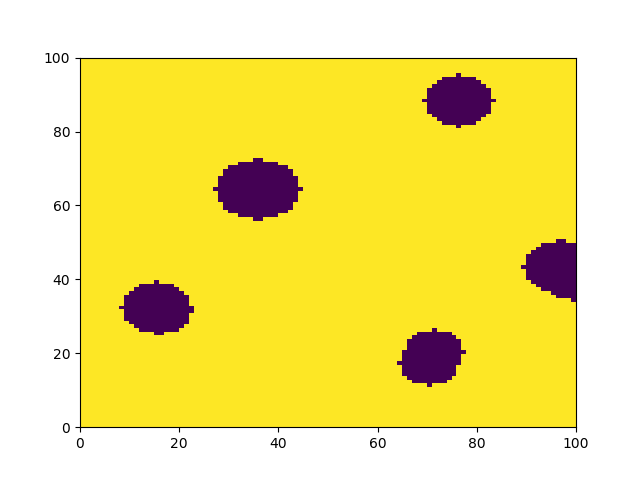
\includegraphics[height=1.2in, width=1.4in]{../BDC_grid2_strongsig}
        \caption{ $k \sim Trun(Poi(50), 1, 100)$; $r \sim TN(7, 2, 5, 10)$; $\beta \sim TN(30, 3, 2, 200)$}
    \end{subfigure}%
        \begin{subfigure}[t]{0.3\textwidth}
        \centering
        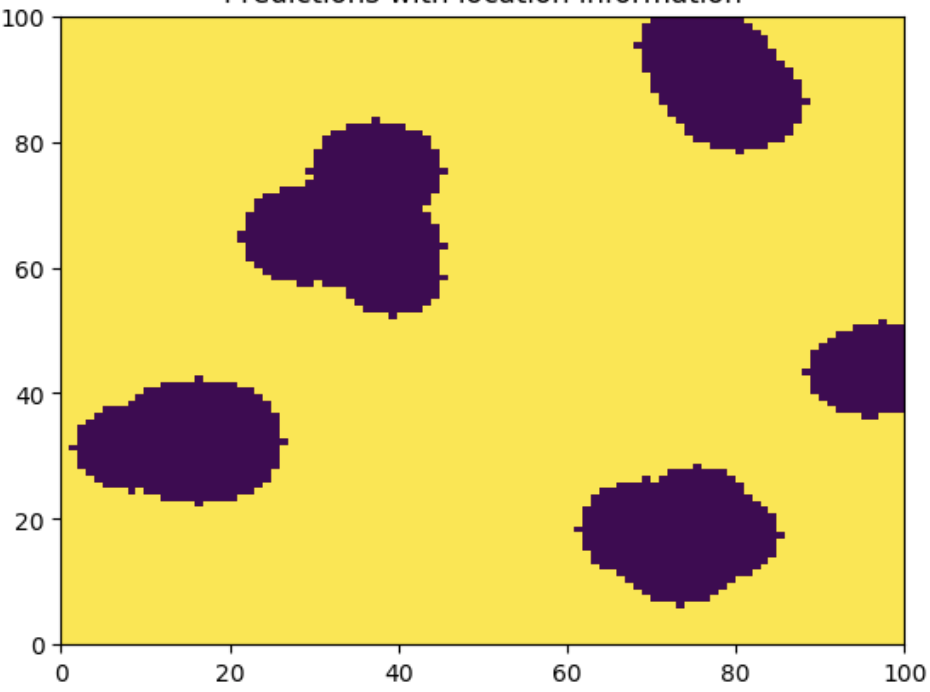
\includegraphics[height=1.2in, width=1.4in]{../BDC_grid3_weaksig}
        \caption{ $k \sim Trun(Poi(50), 1, 100)$; $r \sim TN(7, 2, 5, 10)$; \textbf{$\beta \sim TN(2, 1, 2, 200)$}}
    \end{subfigure}
    \caption{Simulated data}
\end{figure}
\end{frame}

\begin{frame}{Toy Data (continued): More on Priors}
Now, let's compare different priors on radius.
\begin{figure}[t!]
    \centering
    \begin{subfigure}[t]{0.3\textwidth}
        \centering
        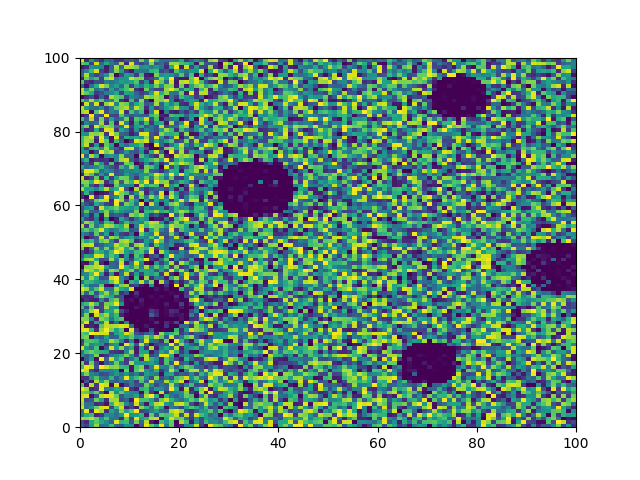
\includegraphics[height=1.3in, width=1.4in]{../BDC_gridactual}
        \caption{Actual grid}
    \end{subfigure}%
    \begin{subfigure}[t]{0.3\textwidth}
        \centering
        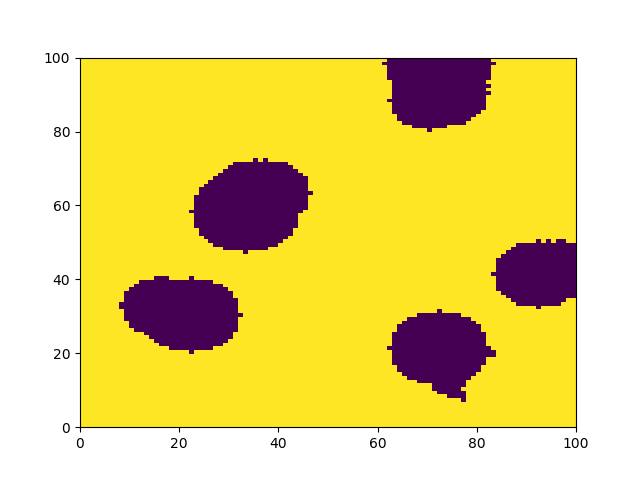
\includegraphics[height=1.2in, width=1.4in]{../BDC_grid4}
        \caption{ $k \sim Trun(Poi(50), 1, 100)$; $r \sim TN(10, 2, 7, 13)$; $\beta \sim TN(8, 5, 2, 200)$}
    \end{subfigure}%
        \begin{subfigure}[t]{0.3\textwidth}
        \centering
        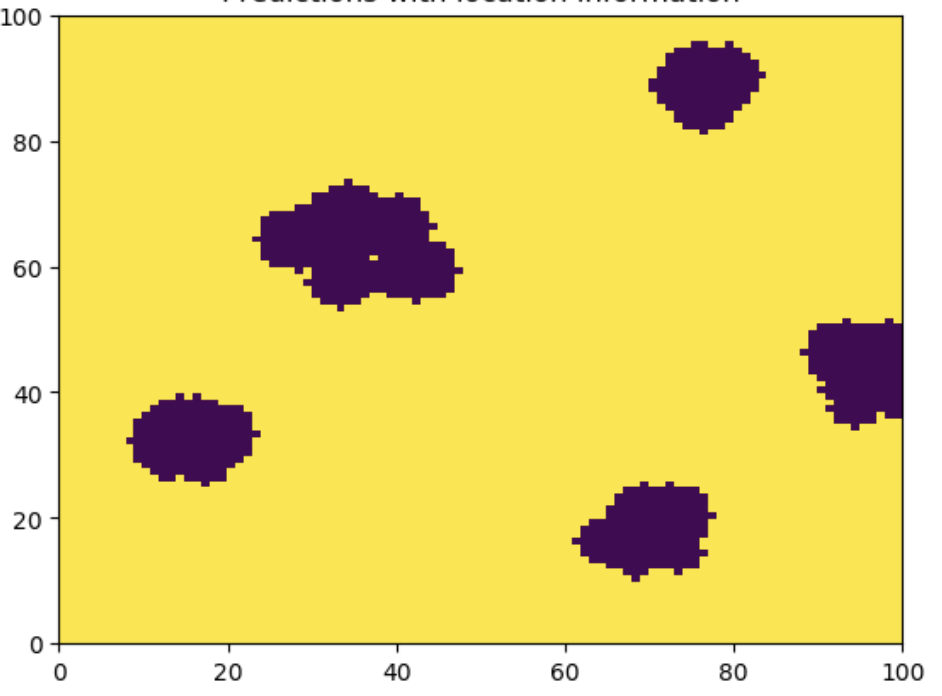
\includegraphics[height=1.2in, width=1.4in]{../BDC_grid5}
        \caption{ $k \sim Trun(Poi(50), 1, 100)$; $r \sim TN(2, 2, 1, 10)$; $\beta \sim TN(8, 5, 2, 200)$}
    \end{subfigure}
    \caption{Simulated data}
\end{figure}
\end{frame}


\begin{frame}{Toy Data (continued): More on Priors}
What if we make signal stronger?
\begin{figure}[t!]
    \centering
    \begin{subfigure}[t]{0.3\textwidth}
        \centering
        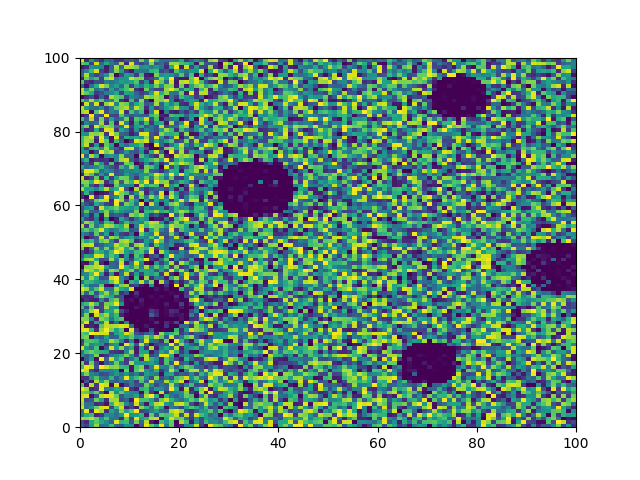
\includegraphics[height=1.3in, width=1.4in]{../BDC_gridactual}
        \caption{Actual grid}
    \end{subfigure}%
    \begin{subfigure}[t]{0.3\textwidth}
        \centering
        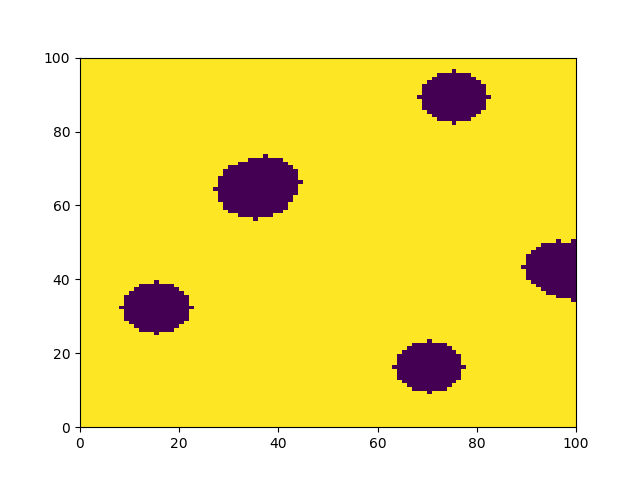
\includegraphics[height=1.2in, width=1.4in]{../BDC_grid4_bigradius_ss}
        \caption{ $k \sim Trun(Poi(50), 1, 100)$; $r \sim TN(10, 2, 7, 13)$; $\beta \sim TN(30, 3, 2, 200)$}
    \end{subfigure}%
        \begin{subfigure}[t]{0.3\textwidth}
        \centering
        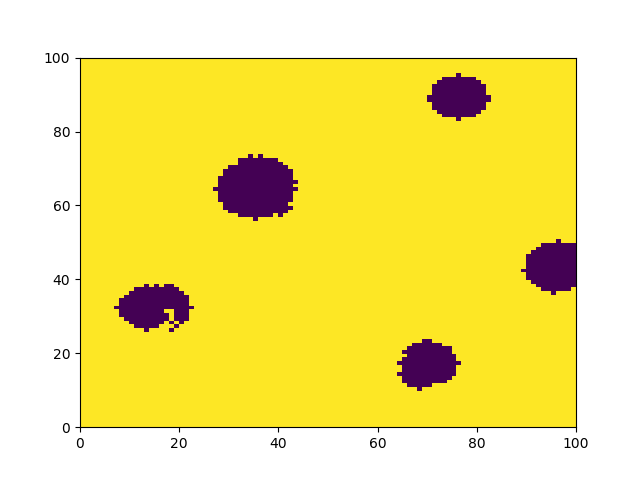
\includegraphics[height=1.2in, width=1.4in]{../BDC_grid5_smallradius_ss}
        \caption{ $k \sim Trun(Poi(50), 1, 100)$; $r \sim TN(2, 2, 1, 10)$; $\beta \sim TN(30, 3, 2, 200)$}
    \end{subfigure}
    \caption{Simulated data}
\end{figure}
\end{frame}


\begin{frame}{Toy Data (continued): More on Priors}
Next, we change the priors on number of clusters.
\begin{figure}[t!]
    \centering
    \begin{subfigure}[t]{0.3\textwidth}
        \centering
        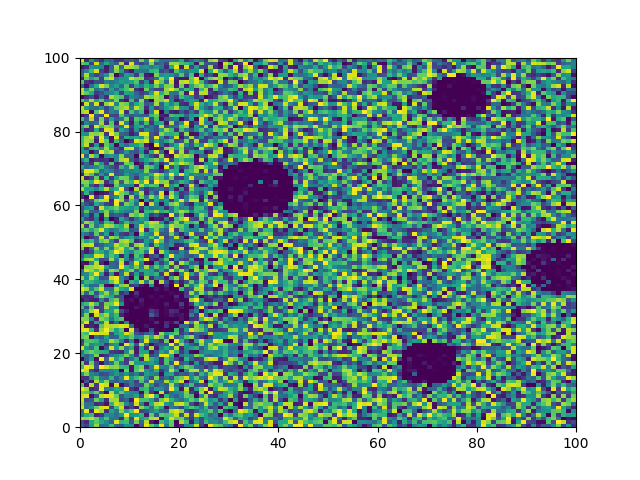
\includegraphics[height=1.3in, width=1.4in]{../BDC_gridactual}
        \caption{Actual grid}
    \end{subfigure}%
    \begin{subfigure}[t]{0.3\textwidth}
        \centering
        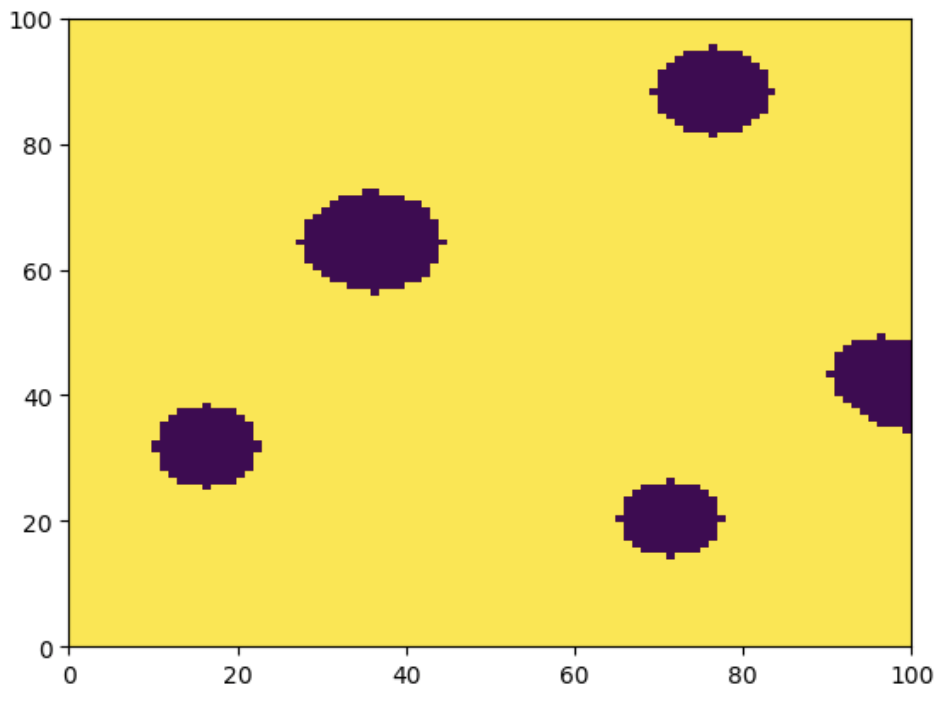
\includegraphics[height=1.2in, width=1.4in]{../BDC_grid7_c3}
        \caption{ $k \sim Trun(Poi(3), 1, 10)$; $r \sim TN(7, 2, 5, 10)$; $\beta \sim TN(8, 5, 2, 200)$}
    \end{subfigure}%
        \begin{subfigure}[t]{0.3\textwidth}
        \centering
        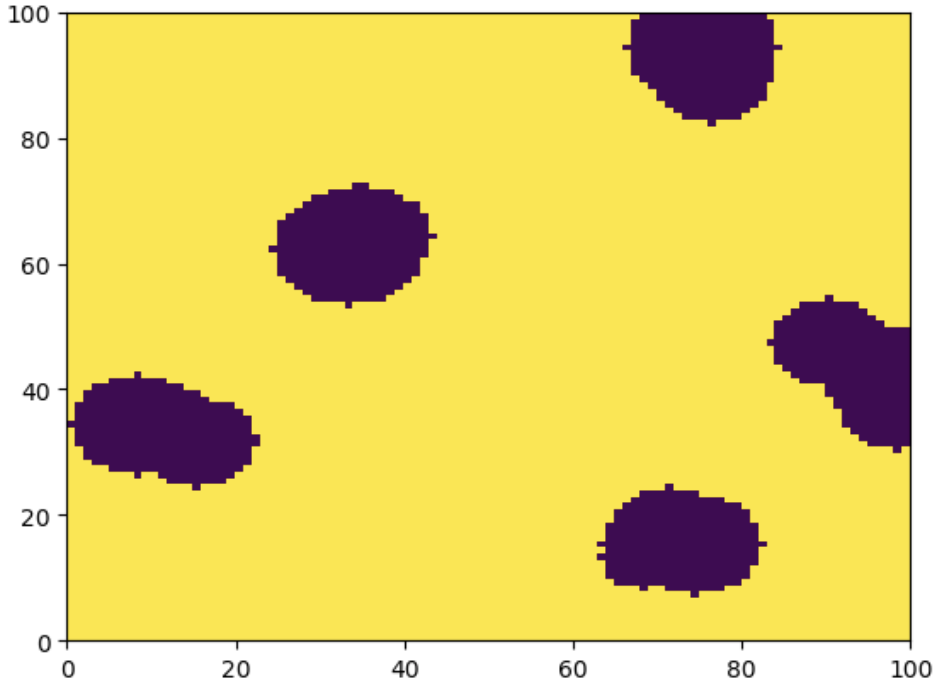
\includegraphics[height=1.2in, width=1.4in]{../BDC_grid8_c300}
        \caption{ $k \sim Trun(Poi(300), 1, 1000)$; $r \sim TN(7, 2, 5, 10)$; $\beta \sim TN(8, 5, 2, 200)$}
    \end{subfigure}
    \caption{Simulated data}
\end{figure}
\end{frame}


\begin{frame}{Toy Data (continued): More on Priors}
Again, let's make signal stronger
\begin{figure}[t!]
    \centering
    \begin{subfigure}[t]{0.3\textwidth}
        \centering
        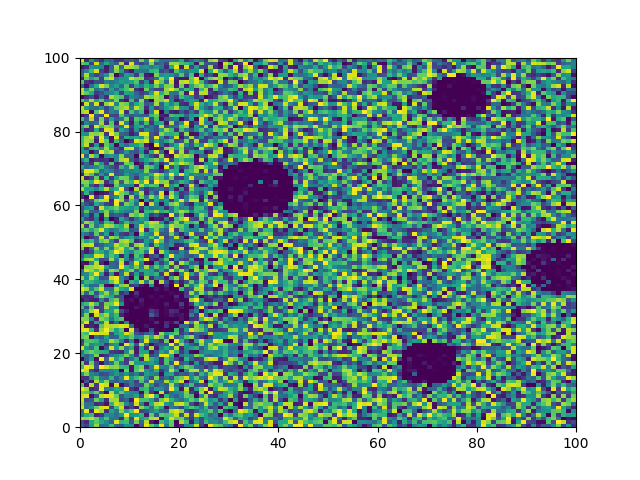
\includegraphics[height=1.3in, width=1.4in]{../BDC_gridactual}
        \caption{Actual grid}
    \end{subfigure}%
    \begin{subfigure}[t]{0.3\textwidth}
        \centering
        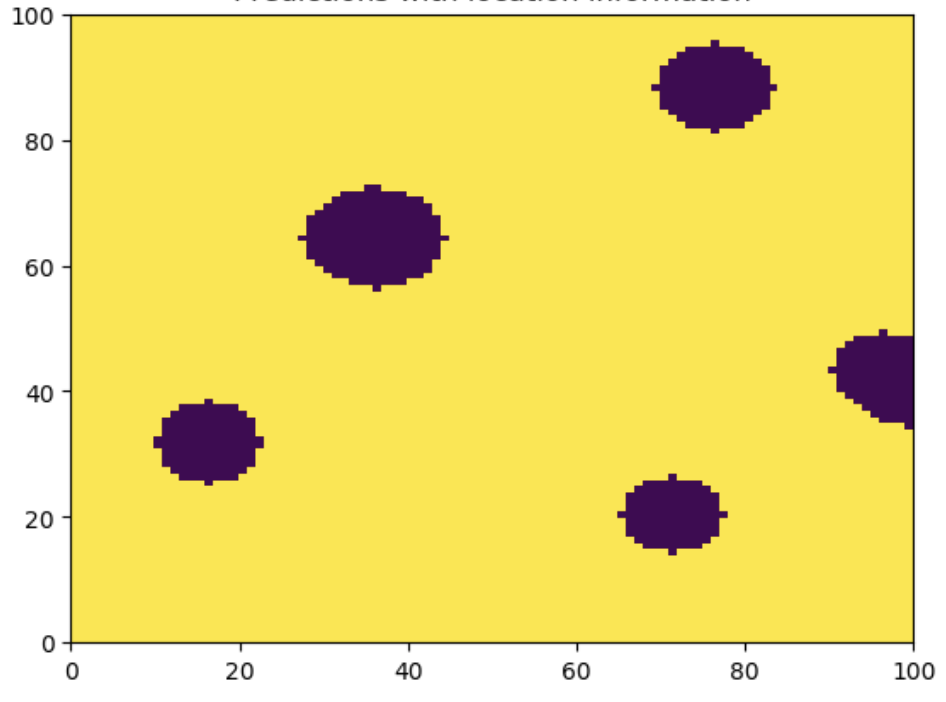
\includegraphics[height=1.2in, width=1.4in]{../BDC_grid7_c3_ss}
        \caption{ $k \sim Trun(Poi(3), 1, 10)$; $r \sim TN(7, 2, 5, 10)$; $\beta \sim TN(30, 3, 2, 200)$}
    \end{subfigure}%
        \begin{subfigure}[t]{0.3\textwidth}
        \centering
        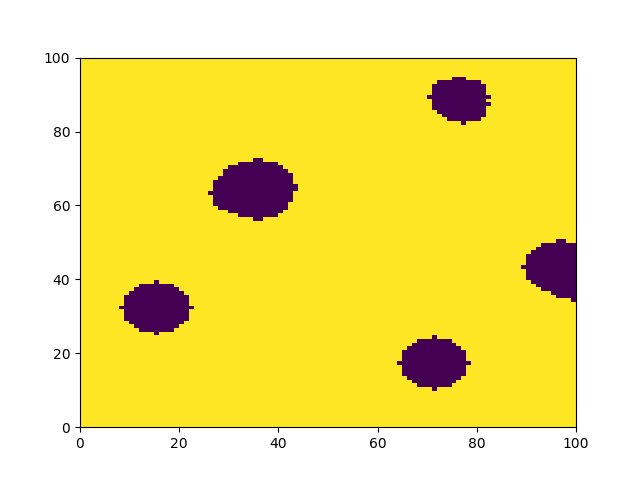
\includegraphics[height=1.2in, width=1.4in]{../BDC_grid8_c300_ss}
        \caption{ $k \sim Trun(Poi(300), 1, 1000)$; $r \sim TN(7, 2, 5, 10)$; $\beta \sim TN(30, 3, 2, 200)$}
    \end{subfigure}
    \caption{Simulated data}
\end{figure}
\end{frame}


\begin{frame}{Toy Data 2 (3-D)}
\begin{figure}[t!]
    \centering
    \begin{subfigure}[t]{0.3\textwidth}
        \centering
        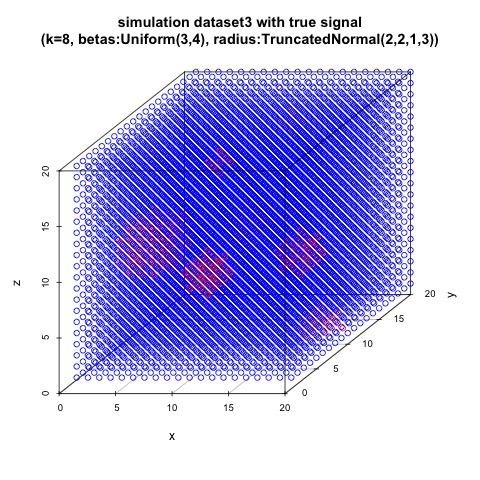
\includegraphics[height=1.4in, width=1.4in]{../simulation_data3.jpg}
        \caption{}
    \end{subfigure}%
    \begin{subfigure}[t]{0.3\textwidth}
        \centering
        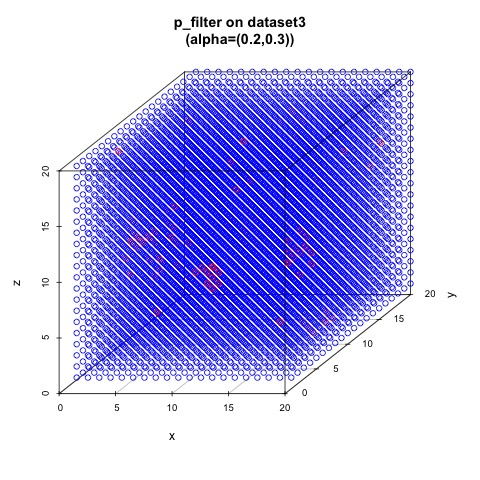
\includegraphics[height=1.4in, width=1.4in]{../p_filterondataset3.jpg}
        \caption{}
    \end{subfigure}%
        \begin{subfigure}[t]{0.3\textwidth}
        \centering
        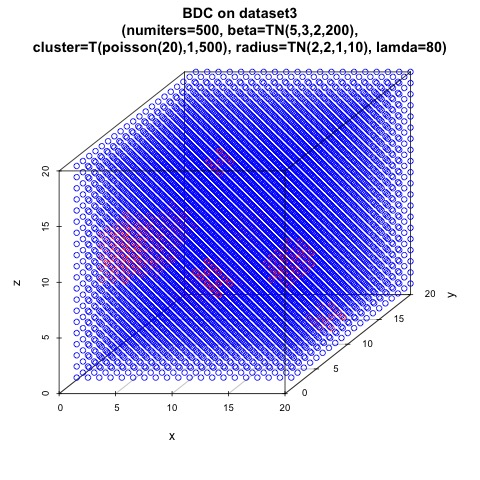
\includegraphics[height=1.4in, width=1.4in]{../best3.jpg}
        \caption{}
    \end{subfigure}
    \caption{Simulated data}
\end{figure}
\end{frame}


\begin{frame}{Toy Data 2 (3-D)}
\begin{figure}[t!]
    \centering
    \begin{subfigure}[t]{0.3\textwidth}
        \centering
        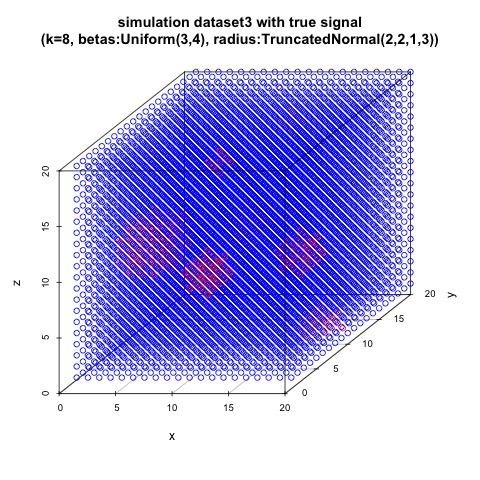
\includegraphics[height=1.4in, width=1.4in]{../simulation_data3.jpg}
        \caption{}
    \end{subfigure}%
    \begin{subfigure}[t]{0.3\textwidth}
        \centering
        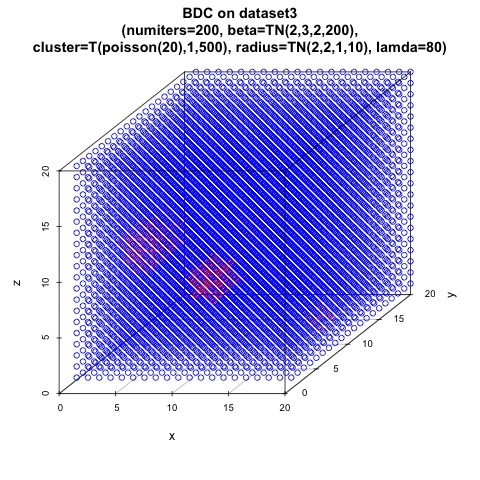
\includegraphics[height=1.4in, width=1.4in]{../dataset3beta3.jpg}
        \caption{}
    \end{subfigure}%
        \begin{subfigure}[t]{0.3\textwidth}
        \centering
        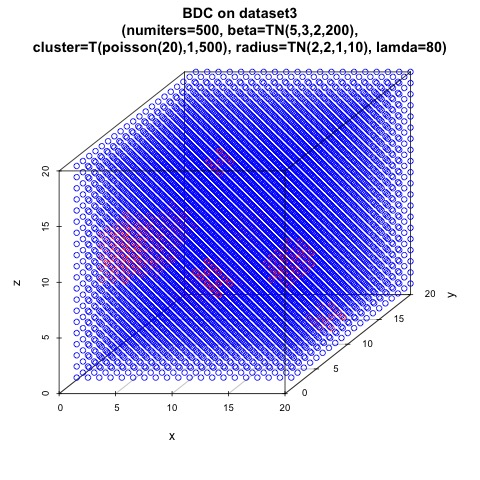
\includegraphics[height=1.4in, width=1.4in]{../best3.jpg}
        \caption{}
    \end{subfigure}
    \caption{Simulated data}
\end{figure}
\end{frame}

\begin{frame}{Toy Data 2 (3-D)}
\begin{figure}[t!]
    \centering
    \begin{subfigure}[t]{0.3\textwidth}
        \centering
        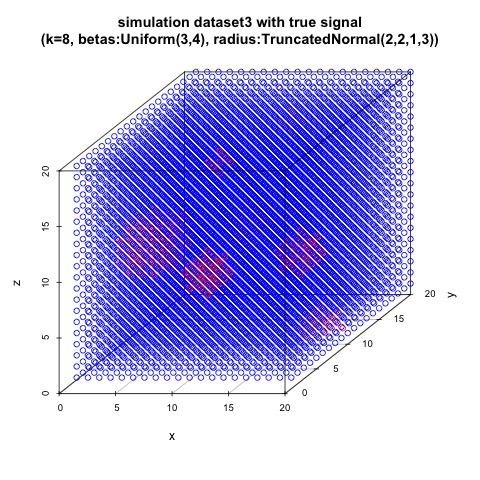
\includegraphics[height=1.4in, width=1.4in]{../simulation_data3.jpg}
        \caption{}
    \end{subfigure}%
    \begin{subfigure}[t]{0.3\textwidth}
        \centering
        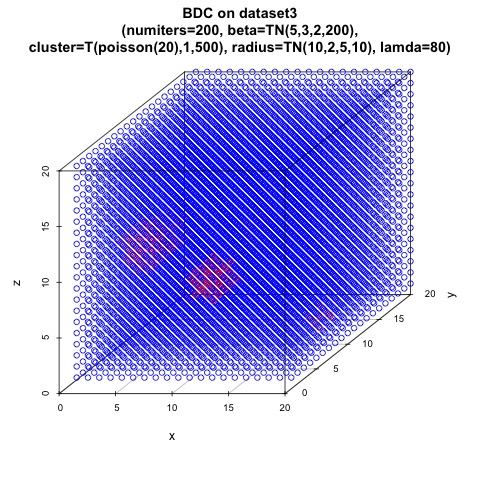
\includegraphics[height=1.4in, width=1.4in]{../radius10.jpg}
        \caption{}
    \end{subfigure}%
        \begin{subfigure}[t]{0.3\textwidth}
        \centering
        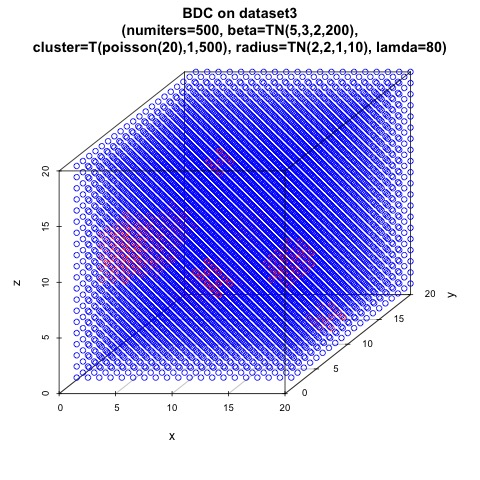
\includegraphics[height=1.4in, width=1.4in]{../best3.jpg}
        \caption{}
    \end{subfigure}
    \caption{Simulated data}
\end{figure}
\end{frame}


\begin{frame}{Toy Data 2 (3-D)}
\begin{figure}[t!]
    \centering
    \begin{subfigure}[t]{0.3\textwidth}
        \centering
        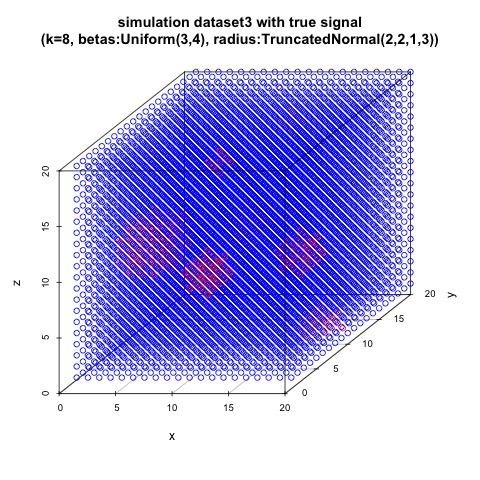
\includegraphics[height=1.4in, width=1.4in]{../simulation_data3.jpg}
        \caption{}
    \end{subfigure}%
    \begin{subfigure}[t]{0.3\textwidth}
        \centering
        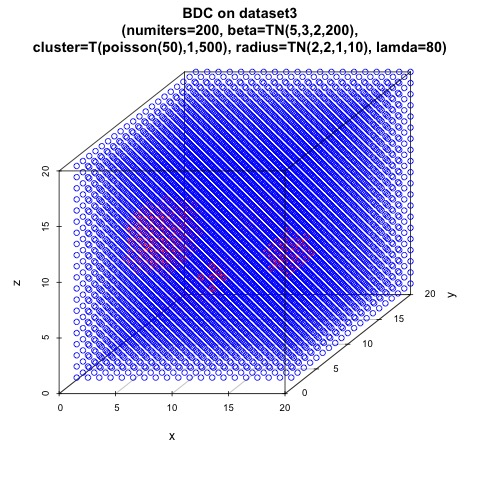
\includegraphics[height=1.4in, width=1.4in]{../datase3_poi50.jpg}
        \caption{}
    \end{subfigure}%
        \begin{subfigure}[t]{0.3\textwidth}
        \centering
        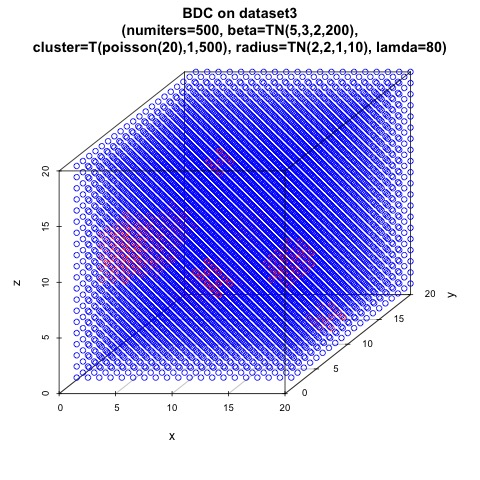
\includegraphics[height=1.4in, width=1.4in]{../best3.jpg}
        \caption{}
    \end{subfigure}
    \caption{Simulated data}
\end{figure}
\end{frame}


\begin{frame}{Performance on real fMRI data}
\begin{figure}[t!]
    \centering
    \begin{subfigure}[t]{0.5\textwidth}
        \centering
        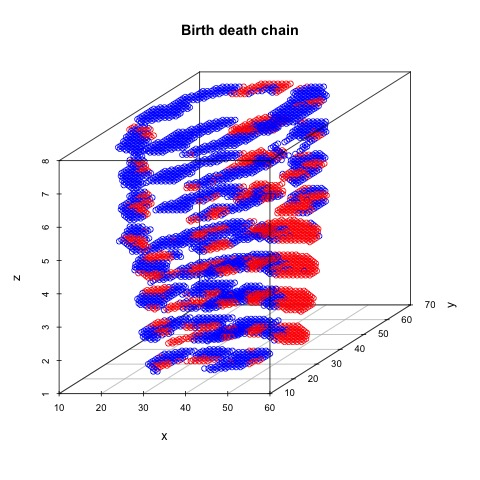
\includegraphics[height=1.8in, width=2in]{../BDC_predictions.jpg}
        \caption{3-D view}
    \end{subfigure}%
    \begin{subfigure}[t]{0.5\textwidth}
        \centering
        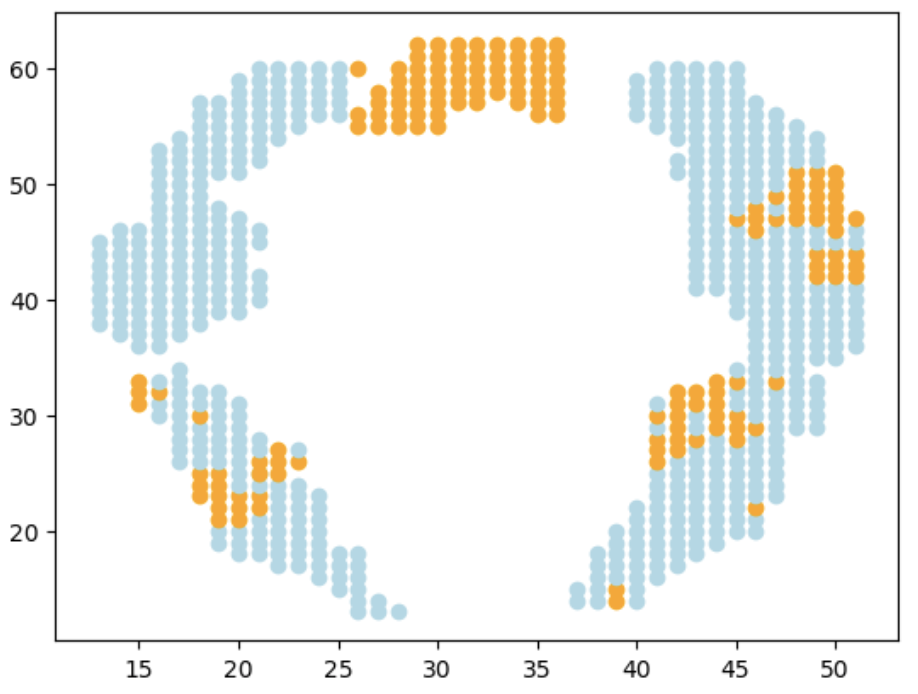
\includegraphics[height=1.2in, width=1.4in]{../BDC_OneSlice}
        \caption{2-D view: one slice}
    \end{subfigure}
    \caption{fMRI data}
\end{figure}
\end{frame}


\begin{frame}{Performance on real fMRI data (continued)}
\centering
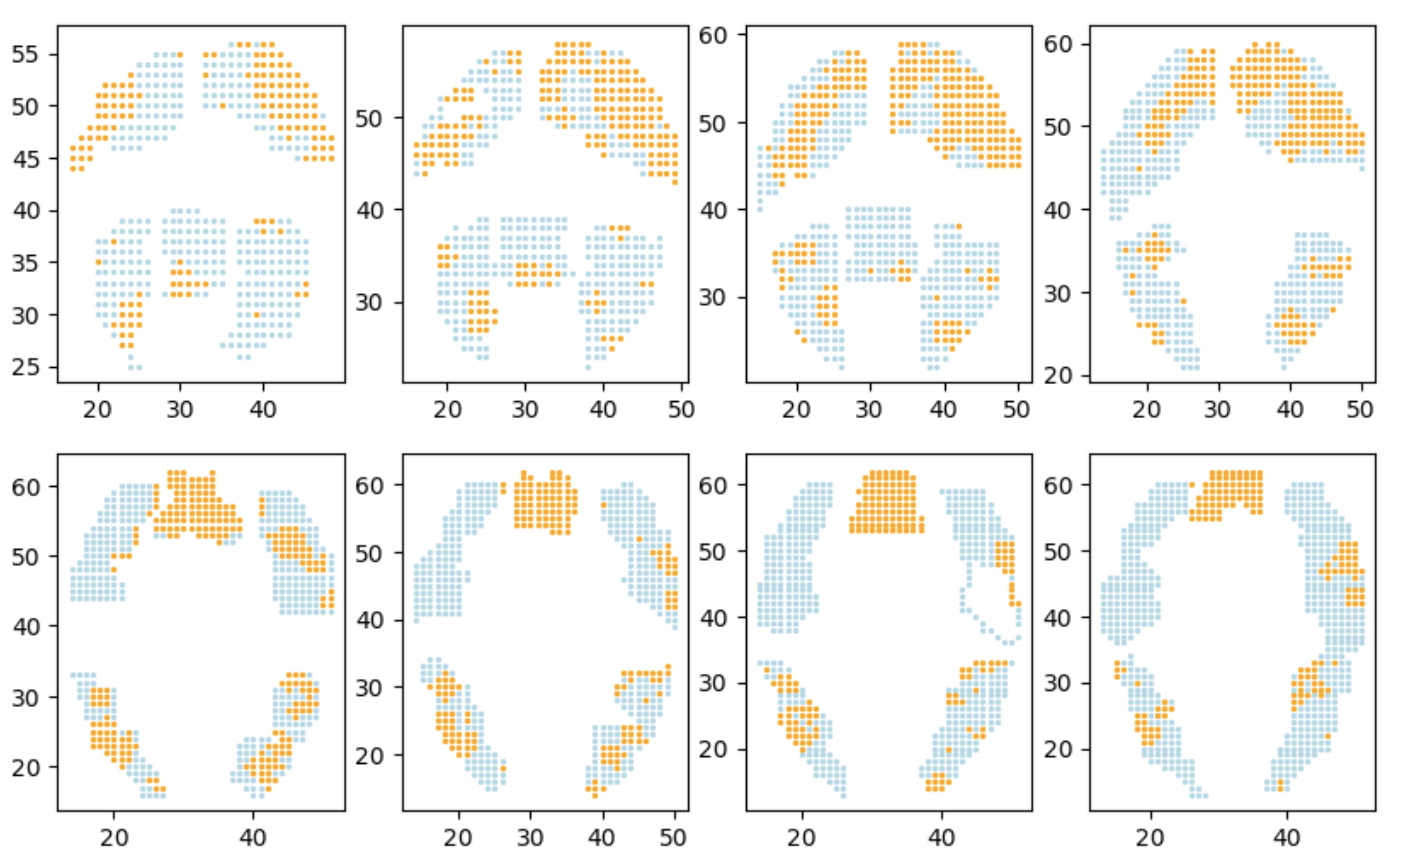
\includegraphics[height=2.5in]{../BDC_AllSlices}
\end{frame}

\begin{frame}{Performance on real fMRI data (continued): Comparison to p-filter}
\begin{figure}[t!]
    \centering
    \begin{subfigure}[t]{0.3\textwidth}
        \centering
        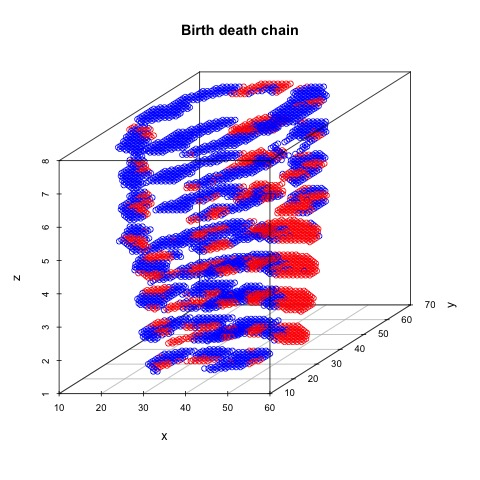
\includegraphics[height=1.4in]{../BDC_predictions.jpg}
        \caption{Birth death chain}
    \end{subfigure}%
    \begin{subfigure}[t]{0.3\textwidth}
        \centering
        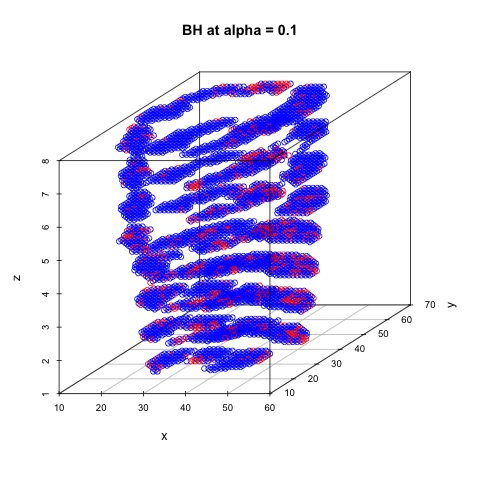
\includegraphics[height=1.4in]{../BH_predictions.jpg}
        \caption{BH}
    \end{subfigure}%
    \begin{subfigure}[t]{0.3\textwidth}
        \centering
        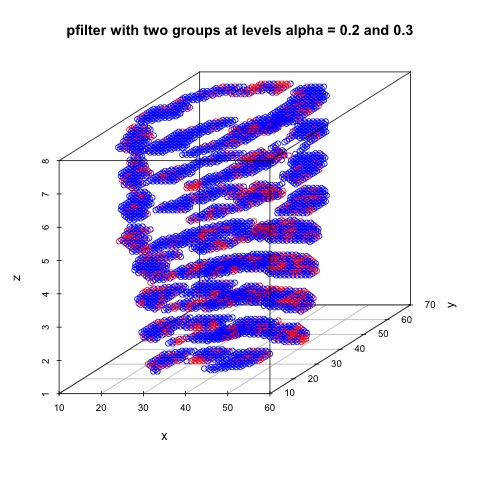
\includegraphics[height=1.4in]{../pfilter_predictions2.jpg}
        \caption{p-filter with $\alpha$ = 0.2,0.3}
    \end{subfigure}
    \caption{fMRI data}
\end{figure}
\end{frame}

\begin{frame}{Conclusion and Future Work}
\BIT
\item Formulated and tested a nonparametric bayesian method to adaptively identify clusters of signals.
\item Showed promising results on both simulation and real fMRI data.
\item Extend from p-values to intensities directly by specifying appropriate priors for null distributions and for signal distributions.
\item Put priors on the hyper-parameters and maximize this priors using EM. That is uniform prior over hyper-parameters.
\EIT
\begin{center}
\textbf{\large Thanks!}
\end{center}
\end{frame}


\end{document}
